\chapter{Introduction}


\chaptermark{intro}
In this thesis we explore several new results relating to the existence of special metrics on certain compact K\"ahler manifolds admitting an effective algebraic torus action. Our goal is to further the understanding of canonical metrics on these types of manifolds. We will do this by finding new examples, and providing novel effective methods of calculating relevant invariants. Our methods are also a concrete demonstration of the power and utility of the language of $T$-varieties.

We begin with a brief primer on the theory for the uninitiated reader. A \textit{K\"ahler manifold} is a smooth manifold \(X\) adorned with mutually compatible Riemannian, complex, and symplectic structures. In this situation we call the Riemannian metric \(g\) the \textit{K\"ahler metric} on \(X\), and the symplectic form \(\omega\) the \textit{K\"ahler form} of \(X\).

There are many reasons to study K\"ahler geometry. From the standpoint of algebraic geometry, every smooth complex projective variety inherits a K\"ahler structure. From a differential geometric perspective, K\"ahler manifolds are a particularly well-behaved class of Riemannian manifolds, and are a rich enough class to contain many interesting examples. There are also motivations from theoretical physics: The various models of our universe in string theory require extra planck-scale dimensions, and certain K\"ahler manifolds are the best candidates for the shape of these dimensions.

Historically, it has been an important problem to investigate which K\"ahler manifolds admit nice K\"ahler metrics. Generally, what we mean here by ``nice" depends on context. For naive motivation consider the real 2-sphere \(S^2\). Most would have in their mind the standard embedding \(S^2 = \{ x^2+y^2+z^2 = 1 \} \subset \RR^3\), see Figure~\ref{fig1a}. There are, however, many choices of smooth embedding, each one corresponding to different choices of Riemannian metrics on \(S^2\), see for example Figure~\ref{fig1b}. What sets our favourite embedding apart is that the induced metric has \textit{constant curvature}.

This is a special case of a wider phenonemon if we identify the sphere as the Riemann surface \(S^2 \cong \PP_\CC^1\). The uniformization theorem, originally proven by Poincar\'e \cite{poincare1908uniformisation} and Koebe \cite{koebe1909uniformisierung, koebe1910uniformisierung}, tells us that any Riemann surface admits a metric of constant scalar curvature. The obvious question is then: What happens in higher dimensions?

%
%\begin{figure*}[h!] \label{fig1}
%    \centering
%    \begin{subfigure}[t]{0.5\textwidth} \label{fig1a}
%        \centering
%        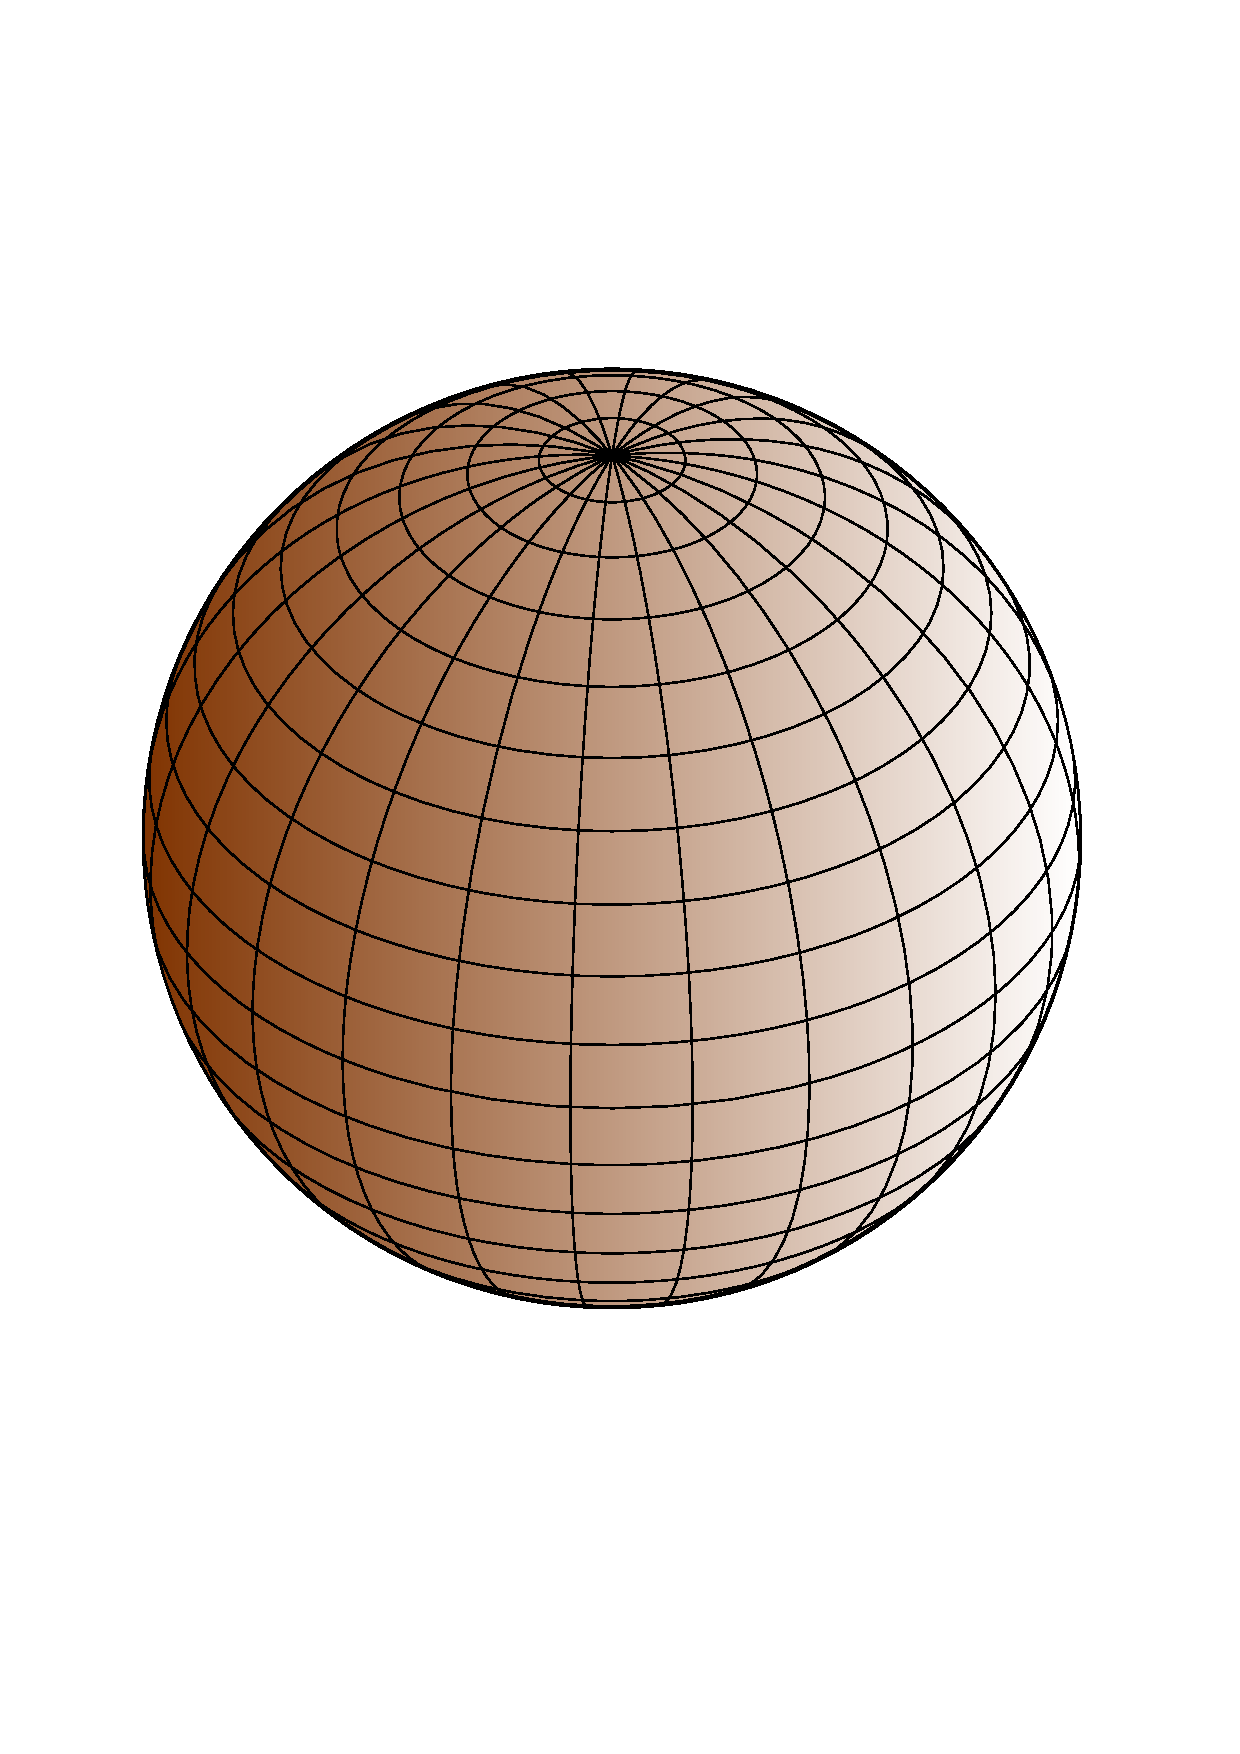
\includegraphics[height=\textwidth]{sphere}
%        \caption{Constant scalar curvature}
%    \end{subfigure}%
%    ~ 
%    \begin{subfigure}[t]{0.5\textwidth} \label{fig1b}
%        \centering
%        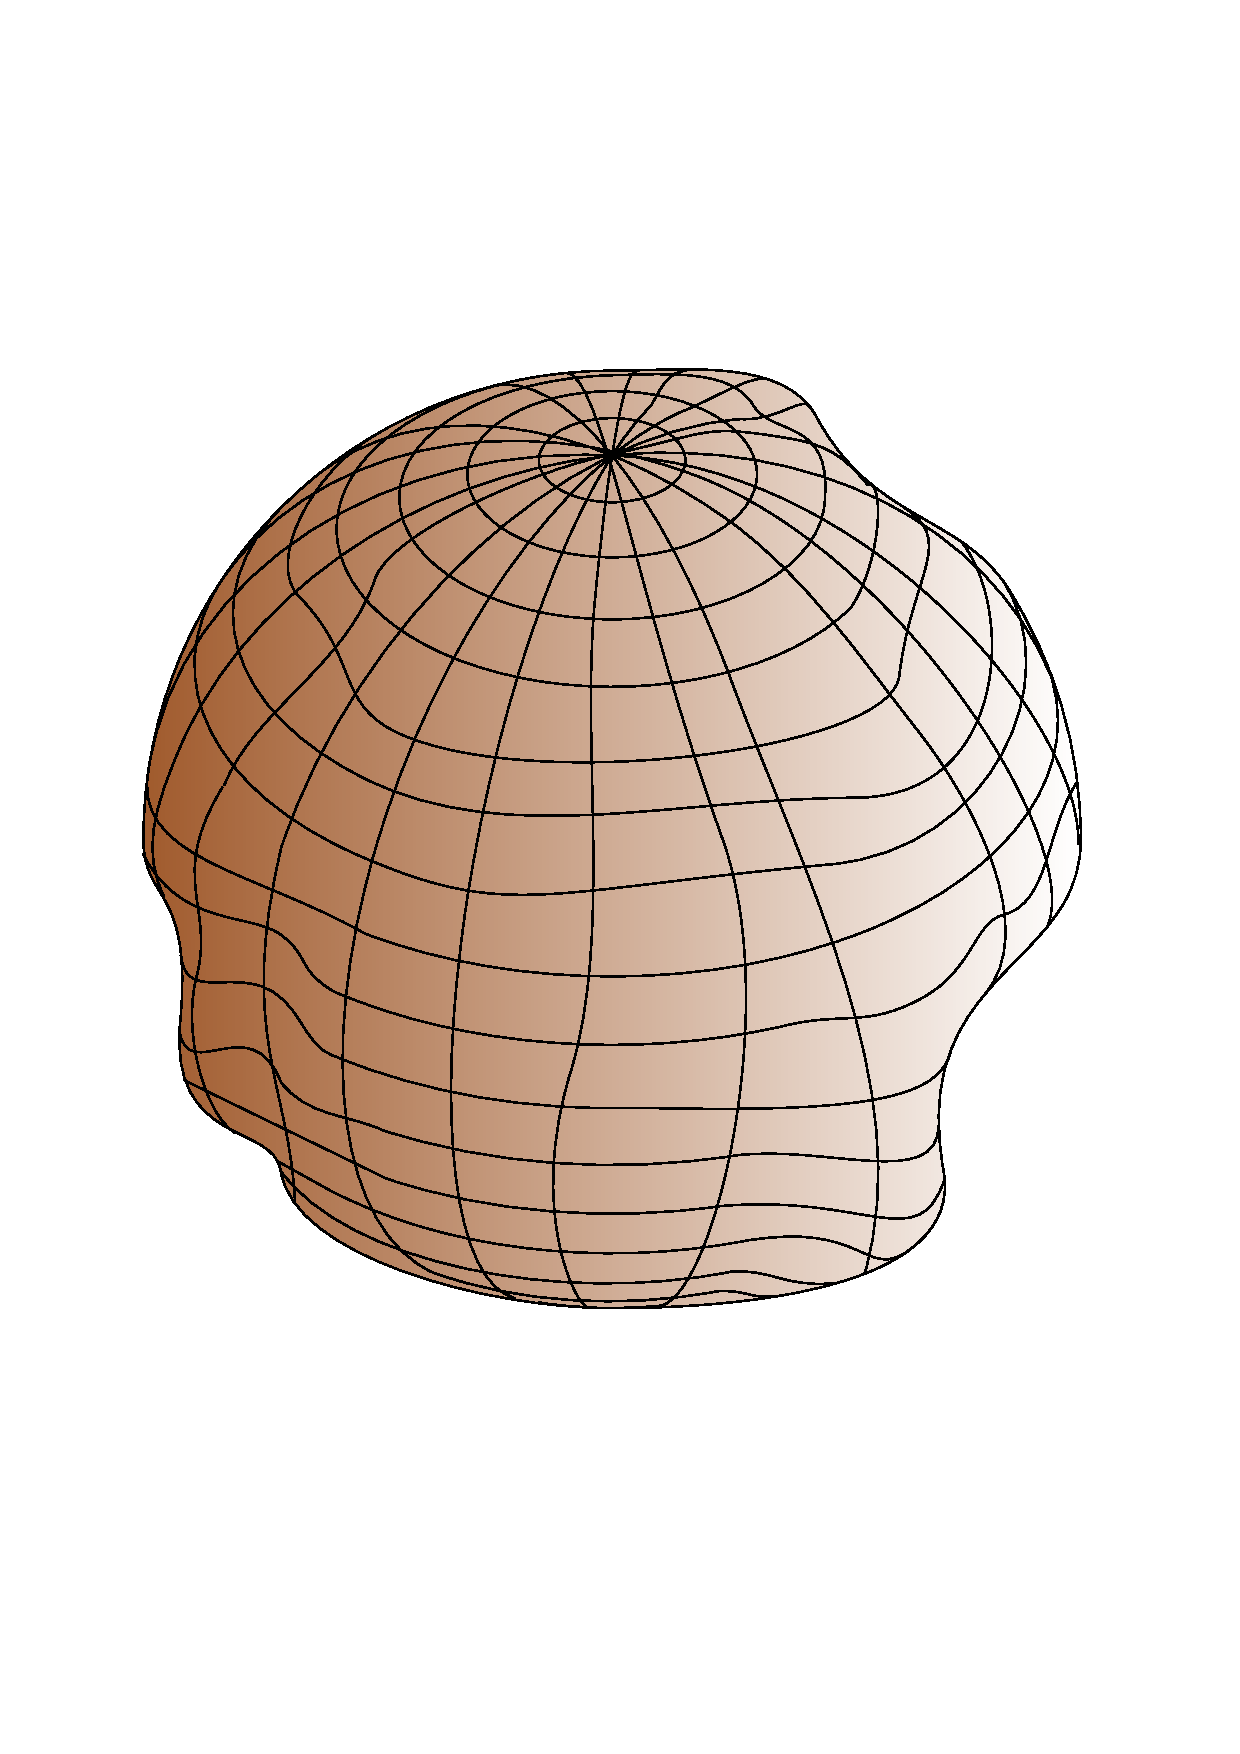
\includegraphics[height=\textwidth]{notsphere}
%        \caption{non-constant scalar curvature}
%    \end{subfigure}
%    \caption{two choices of metric on \(S^2\)}
%\end{figure*}

\begin{figure}[H]
	\subcaptionbox{A metric of constant scalar curvature \label{fig1a}}{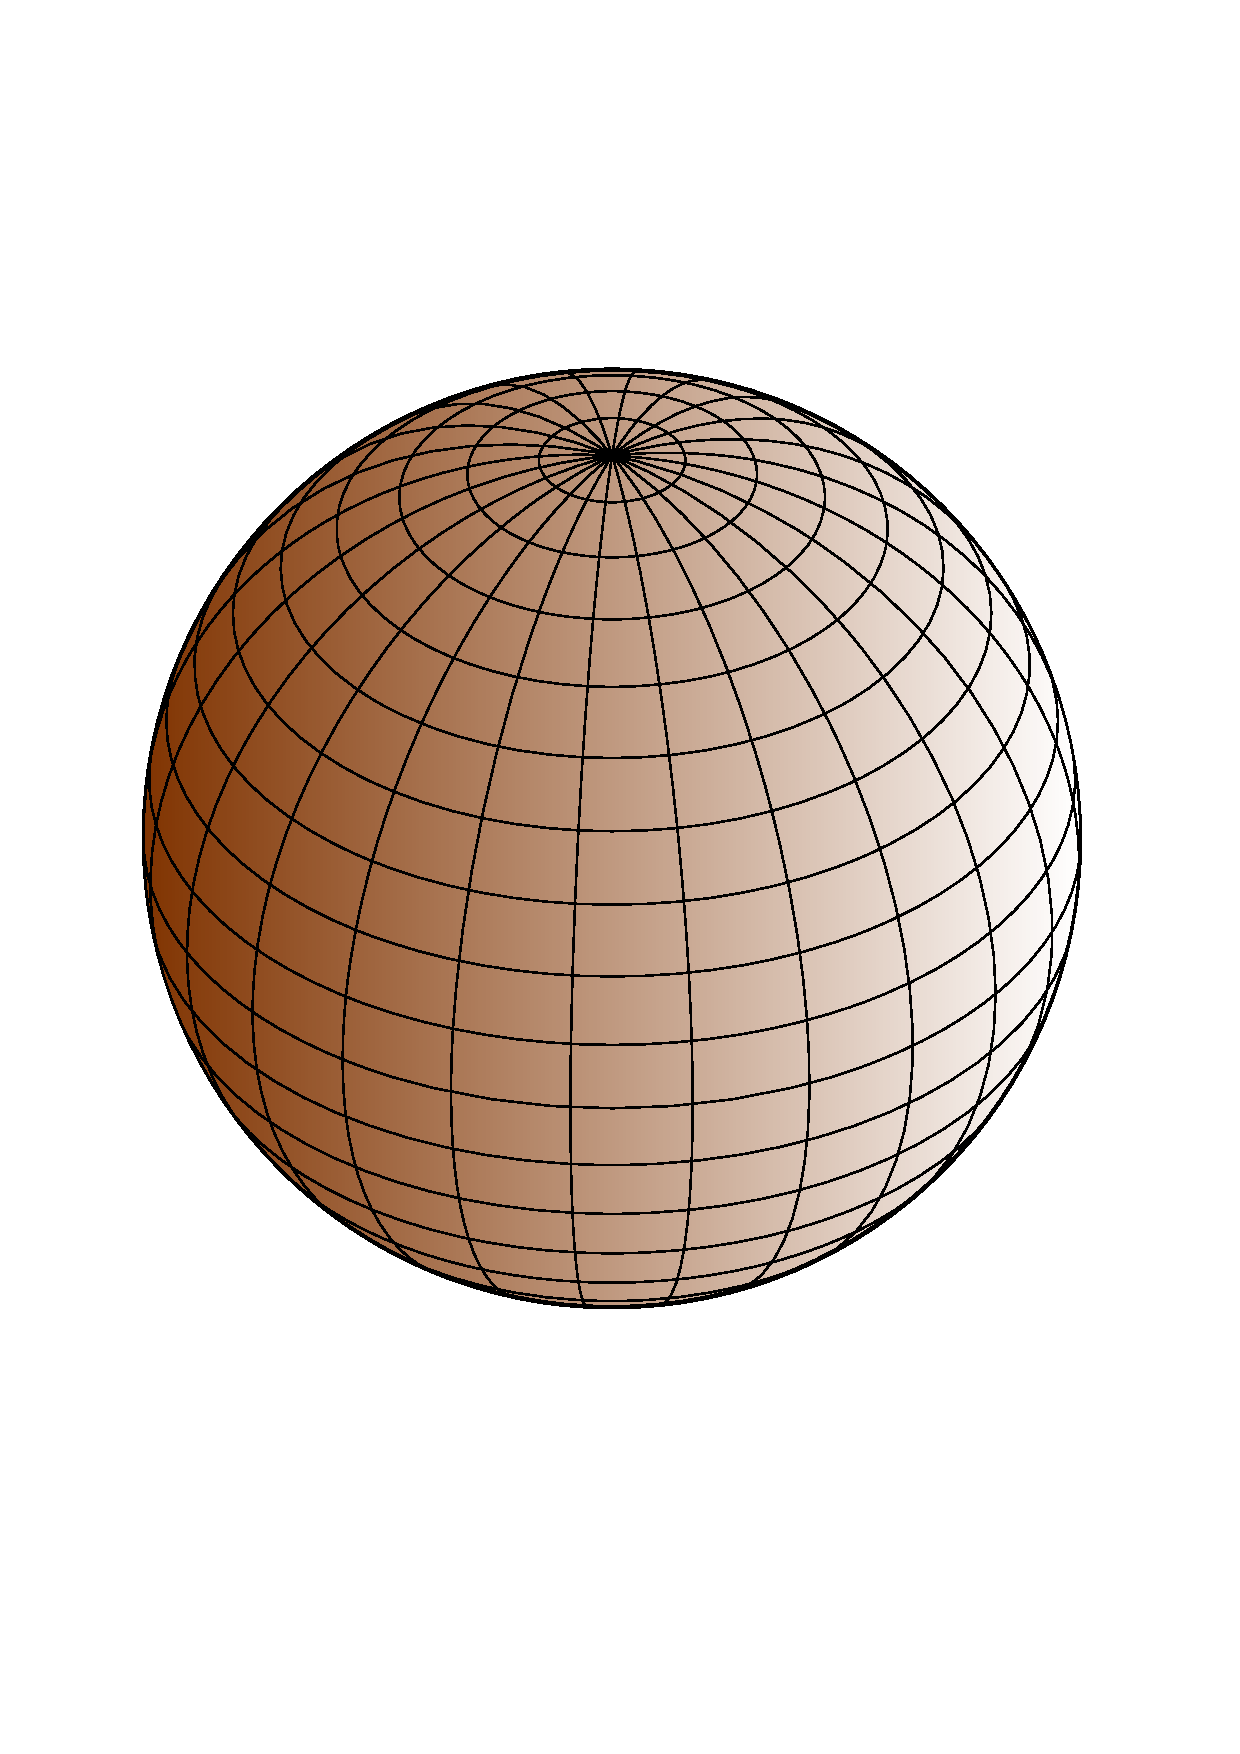
\includegraphics[width=0.45\textwidth]{sphere}}\hfill%
	\subcaptionbox{A metric of non-constant scalar curvature \label{fig1b}}{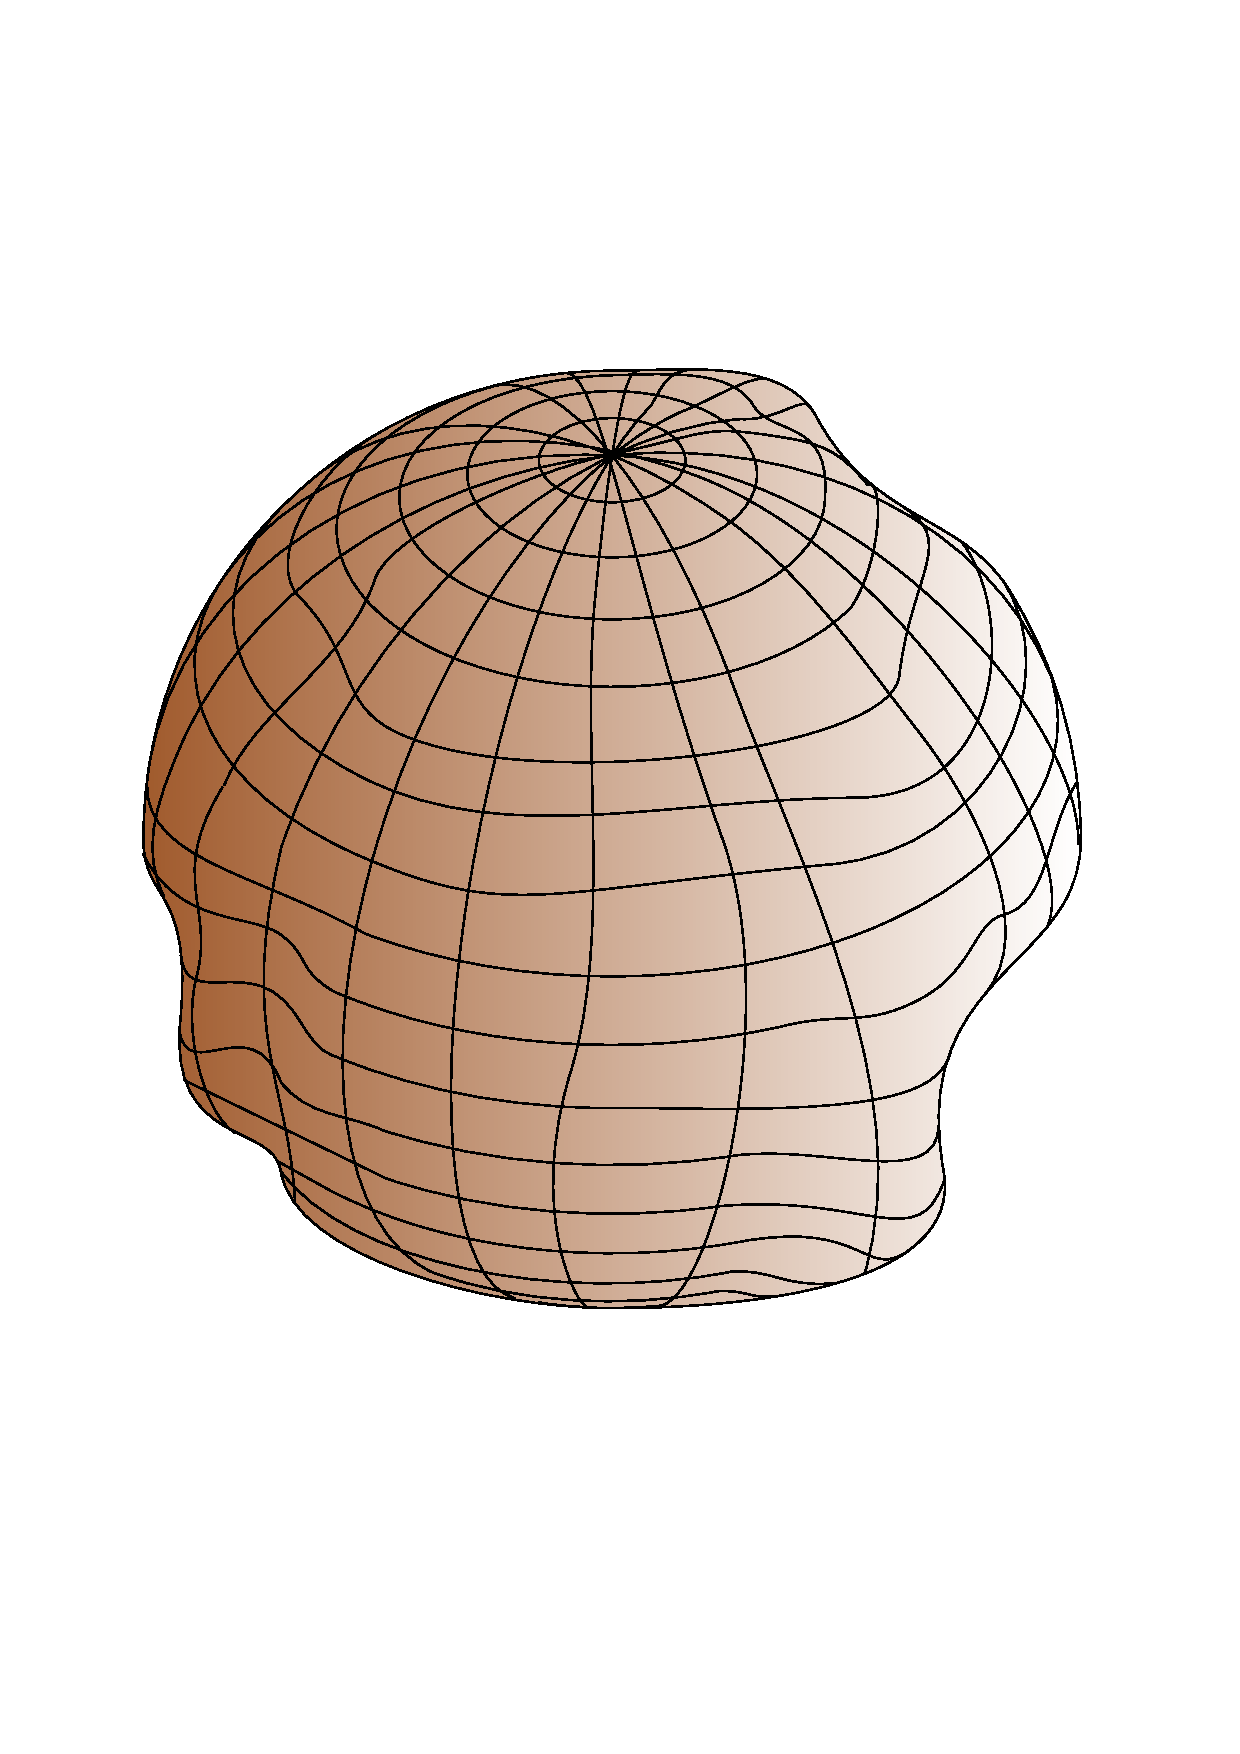
\includegraphics[width=0.45\textwidth]{notsphere}}%
	\caption{Two choices of metric on $S^2$. \label{fig1}}
\end{figure}
In \cite{calabi54,calabi57}, Calabi proved certain results for compact K\"ahler manifolds which lead to a now famous conjecture. Fix a compact K\"ahler manifold \((X,\omega)\). Recall that the Ricci curvature form \(\Ric(\omega)\) is a real \((1,1)\)-form and defines a characteristic class \(c_1(X) = \frac{1}{2 \pi} [ \Ric(\omega)] \) of the manifold, known as the first Chern class. Calabi asked whether, given a real \((1,1)\)-form \( \eta \) representing the first Chern class of \(X\), can we find a unique K\"ahler metric \(\omega'\) in the same cohomology class as \(\omega\) such that \(\Ric(\omega') = 2 \pi \eta\)?

A related conjecture asks whether all compact K\"ahler manifolds \((X,\omega)\) admit a K\"ahler-Einstein metric, or more formally whether they admit a K\"ahler form \(\omega'\) in the same cohomology class as \(\omega\) with \(\Ric \omega' = \lambda \omega'\), for some real constant \(\lambda\). This equation is known as the Einstein condition\footnote{By analogy to Einstein's field equation for a vacuum.}, and the K\"ahler metric corresponding to \(\omega'\) is called a K\"ahler-Einstein metric.

It follows by definition that, for \(X\) to admit such a metric, \(\Ric \omega'\) must be a definite \((1,1)\)-form. This separates the problem into three cases: Where \(\Ric \omega' \) is positive definite, zero, or negative definite. In the first two cases K\"ahler-Einstein metrics on \(X\) are precisely the metrics of constant scalar curvature, and so one may see this as a direct generalization of the uniformization theorem for Riemann surfaces.

Aubin \cite{Aubin1976} and Yau \cite{Yau1977} settled the negative definite case first. Calabi's conjecture was also proven by Yau in \cite{Yau1977}, later contributing to him being awarded the Fields Medal. This left the positive definite case, which corresponds to smooth Fano varieties under the Kodaira embedding theorem. It was already, known however, due to Matsushima \cite{matsushima1957structure}, that not all Fano manifolds were K\"ahler-Einstein. Thus, it became an objective to find suitable criteria for the existence of a K\"ahler-Einstein metric on a Fano manifold.

In \cite{futaki1983obstruction} Futaki introduced a new invariant whose vanishing was also a necessary condition. In \cite{tian1987kahler} Tian introduced a sufficient condition in terms of another invariant, known now as \textit{Tian's alpha invariant}.
Tian's alpha invariant is a generalization of the complex singularity exponent of a polynomial \(f \in \CC[z_1,\dots,z_n]\), which is defined as follows:
\[
c_O(f) := \sup \{ \epsilon | \ |f|^{-2 \epsilon} \text{ integrable  in a neighborhood of } O \in \CC^n \} .
\]
The Yau-Tian-Donaldson conjecture suggested the notion of \textit{ \(K\)-stability} as a necessary and sufficient K\"ahler-Einstein criterion\footnote{In full, the YTD talks of csck metrics, which are equivalent to KE in the Fano case}. This was proven in the trilogy of papers \cite{chen2015kahler1,chen2015kahler2,chen2015kahler3}.

A generalization of the notion of a K\"ahler-Einstein metric is a K\"ahler-Ricci soliton. To understand how, recall that K\"ahler Einstein metrics may be seen as generalized fixed point solutions under the K\"ahler-Ricci flow:
\[
\frac{d}{dt} \omega_t = -2 \Ric(\omega_t),
\]
in that under this flow they will remain unchanged up to some scaling factor. A K\"ahler-Ricci soliton is a generalized fixed point of the flow in the sense that it will remain unchanged up to some biholomorphism.

A further generalization are twisted K\"ahler-Einstein metrics and twisted K\"ahler-Ricci solitons. These arise in continuity method arguments, see \cite{datar2016kahler} for example, and depend on a parameter \(t \in [0,1]\). Here we start with a Calabi-Yau type solution \(\omega_0\) at \(t=0\), and consider the existence of solutions \(\omega_t\) along a line segment to the target K\"ahler-Einstein or K\"ahler-Ricci soliton equation at \(t= 1\) respectively. The supremum of the set of \(t\) for which a solution exists turns out to be independent of \(\omega_0\), and is of interest as an invariant of \(X\). It is known as \textit{Tian's beta invariant}, or the \textit{greatest lower bound on Ricci curvature}. We will denote this invariant by \(R(X)\).

Although \(K\)-stability is a criterion for the existence of K\"ahler-Einstein metrics and their various generalizations, it is not an effective one. In general, the \(K\)-stability of a Fano manifold is difficult to calculate. The alpha invariant approach also has limitations in practice. Fortunately, equivariant versions of \(K\)-stability and Tian's alpha invariant exist, which, as we will see, provide an effective approach in classes of manifolds and orbifolds with a high degree of symmetry.

In this thesis we will focus our attention on Fano manifolds which are also \textit{\(T\)-varieties}. A \(T\)-variety is a normal variety which admits an effective action of an algebraic torus \(T = (\CC^*)^r\). These are a generalization of toric varieties, where \(\dim T = \dim X\). In general we call the difference \(\dim X - \dim T\) the \textit{complexity} of the torus action.

In the toric case it is well-established that studying \(X\) is equivalent to studying some associated combinatorial data: a fan of cones in a vector space built from the cocharacter lattice of \(T\). Thanks to the work of many authors (Altmann, Hausen, Ilten, Petersen, S\"u\ss, Vollmert, Liendo to name a few) this combinatorial description extends to higher complexity. We recall some of the theory in Chapter~\ref{chap:prelim}.

Equivariant methods have been used to provide some effective criteria for canonical metrics on low complexity \(T\)-varieties. If \(X\) is a Fano toric variety then the K\"ahler-Einstein problem is completely solved. In \cite{wang2004} it was shown that \(X\) is K\"ahler-Einstein if and only if the Futaki character vanishes. They also showed that the Futaki character coincides with the barycenter of the lattice Polytope corresponding to \(X\). Wang et al did not use \(K\)-stability for this result, but the result was later reproven as an application of the main theorem of \cite{datar2016kahler}.

In \cite{ilten2015}, S{\"u}{\ss} and Ilten considered the \(K\)-stability of \(T\)-varieties of complexity one. We recall this in detail in Section~\ref{prelim:twisted}. They obtained a combinatorial criterion for \(K\)-stability, generalizing the results of \cite{wang2004}. S{\"u}{\ss} had also used the equivariant version of Tian's alpha invariant to find new K\"ahler-Einstein metrics on complexity one \(T\)-varieties admitting additional symmetries in \cite{suss2013kahler}.

In complexity two and above, even equivariant \(K\)-stability remains an ineffective criterion. There is, as we shall see, scope for methods like that of \cite{suss2013kahler}. In the next section we will give an overview of the content of this thesis.

\section{Content of the Thesis} \label{content}
Here we summarize the remaining structure of the thesis. Some of the content of this thesis has been published, and/or submitted to journals. I reference relevant sources clearly when this is the case. I also make clear, in the case of my coauthored work in Chapter 3, the scope of my contribution to the original paper.
\subsection*{Chapter 2 - Preliminaries}
We recall definitions and results from K\"ahler, algebraic, and symplectic geometry to give context to our novel results. We then give a brief introduction to the theory of \(T\)-varieties and their equivariant \(K\)-stability, which are key in our methods of proof in Chapters 3 and 4.
\subsection*{Chapter 3 - New K\"ahler-Ricci solitons on Fano threefolds} \label{content:riccisolitons}
In Chapter~\ref{chap:sol} we consider Fano threefolds admitting an effective \(2\)-torus action within the classification of \cite{mori1981classification}. In \cite{suss2013fano} a not necessarily complete list of such threefolds together with their combinatorial description was given. We extend the results of \cite{ilten2015}, providing new examples of threefolds admitting a non-trivial K\"ahler-Ricci soliton. Recall that a K\"ahler-Ricci soliton on a Fano manifold \((X,\omega)\) is a pair \((\omega',v)\) satisfying:
\[
\Ric(\omega') - L_v \omega' = \omega'
\]
We apply some real interval arithmentic approximations to the complexity one formula for the Futaki invariant of Ilten and S{\"u}{\ss} (see Section~\ref{subsec:IS}) to check the existence criterion \cite{datar2016kahler} (see Section~\ref{prelim:twisted}). We include the relevant Sagemath code in Appendix~\ref{App:code}.
\subsection*{Chapter 4 - The greatest lower bound on Ricci curvature in complexity one} \label{content:R(X)}
In Chapter~\ref{chap:R(X)} we present an explicit effective formula obtained for the greatest lower bound on Ricci curvature \(R(X)\) for a complexity one \(T\)-variety \(X\). We follow the author's work \cite{cable2019greatest}. These results generalize a result of Li \cite{li2009greatest}, but the proof uses results of \(G\)-equivariant \(K\)-stability from \cite{datar2016kahler}. The invariant \(R(X)\) is often denoted \(\beta(X)\) and is referred to as \textit{Tian's beta invariant}. By \cite{} it is now known to coincide with another important invariant, \(\delta(X)\).
\subsection*{Chapter 5 - New K\"ahler-Einstein metrics on symmetric general arrangement varieties} \label{content:generalarrangement}
In Chapter~\ref{chap:gav}, we discuss recent results obtaining new K\"ahler-Einstein metrics on some symmetric complexity two general arrangement varieties. General arrangement varieties are \(T\)-varieties where the torus quotient is a projective space, and the critical values of the quotient map form a general arrangement of hyperplanes in that projective space. Smooth general arrangement varieties of complexity and Picard rank \(2\) were classified according to their Cox ring in \cite{hausen2018torus}. Following the methods of \cite{Su13}, we find three new examples of K\"ahler-Einstein metrics. As far as we are aware, these are the first examples of K\"ahler-Einstein metrics found on \(T\)-varieties of complexity greater than one by way of equivariant methods.